% Source PDF page 599 (printed p. 585), section 11.5 begins here.
\section{基于自协调性的复杂度分析}
利用自协调函数的牛顿法复杂度分析（第9.6.4节，第503页；第10.2.4节，第531页），可以分析障碍法的复杂度。这种分析适用于许多常见问题，并得到几个有意思的结论：它严格给出用障碍法求解问题所需总牛顿步数的上界，并说明为何中心化问题不会随着 $t$ 增大而变得更困难。

% Source PDF page 600 (printed p. 586)
\subsection{自协调性假设}
作以下两个假设。
\begin{itemize}
\item 对所有 $t\ge t^{(0)}$，函数 $tf_0+\phi$ 为闭函数且自协调。
\item 问题 (11.1) 的下水平集有界。
\end{itemize}
第二个假设说明中心化问题的下水平集有界（见习题11.3），因此中心化问题可解。下水平集有界还意味着 $tf_0+\phi$ 的 Hessian 矩阵处处正定（见习题11.14）。虽然自协调性假设将复杂度分析限制在一类特定问题上，但应当强调，无论这一假设是否成立，障碍法一般都能很好地工作。

许多问题满足自协调性假设，包括所有线性问题和二次问题。若函数 $f_i$ 为线性或二次函数，则
\[
tf_0-\sum_{i=1}^m\log(-f_i)
\]
对所有 $t\ge0$ 都自协调（见第9.6节）。因此下面的复杂度分析适用于 LP、QP 和 QCQP。

有时可以重新表述问题，使其满足自协调性假设。例如，考虑线性不等式约束熵最大化问题
\[
\begin{aligned}
\text{最小化}\quad&\sum_{i=1}^n x_i\log x_i\\
\text{约束为}\quad&Fx\preceq g,\\&Ax=b.
\end{aligned}
\]
函数
\[
tf_0(x)+\phi(x)=t\sum_{i=1}^n x_i\log x_i-\sum_{i=1}^m\log(g_i-\bar f_i^\T x),
\]
其中 $\bar f_1^\T,\ldots,\bar f_m^\T$ 是 $F$ 的各行，它不是闭函数（除非 $Fx\preceq g$ 蕴含 $x\succeq0$），也不自协调。但可以增加冗余不等式约束 $x\succeq0$，得到等价问题
\begin{equation}\begin{aligned}
\text{最小化}\quad&\sum_{i=1}^n x_i\log x_i\\
\text{约束为}\quad&Fx\preceq g,\\&Ax=b,\\&x\succeq0.
\end{aligned}\tag{11.23}\end{equation}
此时有
\[
tf_0(x)+\phi(x)=t\sum_{i=1}^n x_i\log x_i-\sum_{i=1}^n\log x_i-\sum_{i=1}^m\log(g_i-\bar f_i^\T x),
\]
% Source PDF page 601 (printed p. 587)
对任意 $t\ge0$，它都是自协调闭函数。（对所有 $t\ge0$，函数 $ty\log y-\log y$ 在 $\R_{++}$ 上自协调；见习题11.13。）因此，复杂度分析适用于重新表述后的线性不等式约束熵最大化问题 (11.23)。

再看一个更特殊的例子，考虑 GP
\[
\begin{aligned}
\text{最小化}\quad&f_0(x)=\log\sum_{k=1}^{K_0}\exp(a_{0k}^\T x+b_{0k})\\
\text{约束为}\quad&\log\sum_{k=1}^{K_i}\exp(a_{ik}^\T x+b_{ik})\le0,\quad i=1,\ldots,m.
\end{aligned}
\]
尚不清楚函数
\begin{align*}
tf_0(x)+\phi(x)={}&t\log\left(\sum_{k=1}^{K_0}\exp(a_{0k}^\T x+b_{0k})\right)\\
&-\sum_{i=1}^m\log\left(-\log\sum_{k=1}^{K_i}\exp(a_{ik}^\T x+b_{ik})\right)
\end{align*}
是否自协调，因此，尽管障碍法有效，本节的复杂度分析却不一定成立。

不过，可以把 GP 重新表述为明确满足自协调性假设的形式。对每一项（单项式）$\exp(a_{ik}^\T x+b_{ik})$，引入新变量 $y_{ik}$ 作为上界：
\[
\exp(a_{ik}^\T x+b_{ik})\le y_{ik}.
\]
用这些新变量，可将 GP 写为
\[
\begin{aligned}
\text{最小化}\quad&\sum_{k=1}^{K_0}y_{0k}\\
\text{约束为}\quad&\sum_{k=1}^{K_i}y_{ik}\le1,\quad i=1,\ldots,m,\\
&a_{ik}^\T x+b_{ik}-\log y_{ik}\le0,\quad i=0,\ldots,m,\quad k=1,\ldots,K_i,\\
&y_{ik}\ge0,\quad i=0,\ldots,m,\quad k=1,\ldots,K_i.
\end{aligned}
\]
对应的对数障碍为
\[
\sum_{i=0}^m\sum_{k=1}^{K_i}\bigl(-\log y_{ik}-\log(\log y_{ik}-a_{ik}^\T x-b_{ik})\bigr)
-\sum_{i=1}^m\log\left(1-\sum_{k=1}^{K_i}y_{ik}\right),
\]
它是自协调闭函数（例9.8，第500页）。由于目标为线性函数，对任意 $t$，$tf_0+\phi$ 都是自协调闭函数。

\subsection{每次中心化的牛顿迭代次数}
第9.6.4节（第503页）和第10.2.4节（第531页）中建立的自协调函数牛顿法复杂度理论表明，最小化严格凸、自协调闭函数 $f$ 所需的牛顿迭代次数，上界为
\begin{equation}
\frac{f(x)-p^\star}{\gamma}+c.\tag{11.24}
\end{equation}
% Source PDF page 602 (printed p. 588)
其中 $x$ 是牛顿法的初始点，$p^\star=\inf_x f(x)$ 是最优值。常数 $\gamma$ 只依赖回溯参数 $\alpha$ 和 $\beta$，由下式给出：
\[
\frac1\gamma=\frac{20-8\alpha}{\alpha\beta(1-2\alpha)^2}.
\]
常数 $c$ 只依赖容差 $\epsilon_{\mathrm{nt}}$，
\[
c=\log_2\log_2(1/\epsilon_{\mathrm{nt}}),
\]
可以合理地用 $c=6$ 近似。式 (11.24) 是一个相当保守的牛顿步数上界，但本节只关心建立复杂度界，重点考察它怎样随问题规模与算法参数增长。

本节用这一结果推导障碍法一次外迭代所需的牛顿步数界，也就是从 $x^\star(t)$ 出发计算 $x^\star(\mu t)$ 的步数界。为简化记号，用 $x$ 表示当前迭代点 $x^\star(t)$，用 $x^+$ 表示下一个迭代点 $x^\star(\mu t)$，用 $\lambda$、$\nu$ 分别表示 $\lambda^\star(t)$、$\nu^\star(t)$。

自协调性假设说明，
\begin{equation}
\frac{\mu t f_0(x)+\phi(x)-\mu t f_0(x^+)-\phi(x^+)}{\gamma}+c\tag{11.25}
\end{equation}
是从 $x=x^\star(t)$ 出发计算 $x^+=x^\star(\mu t)$ 所需牛顿步数的上界。遗憾的是，在实际算出 $x^+$，即执行牛顿算法之前，不知道 $x^+$，也就不知道上界 (11.25)；而执行之后，已经知道计算 $x^\star(\mu t)$ 所需的准确步数，这就失去了求上界的意义。但可以如下推导 (11.25) 的上界：
\begin{align*}
&\mu t f_0(x)+\phi(x)-\mu t f_0(x^+)-\phi(x^+)\\
&=\mu t f_0(x)-\mu t f_0(x^+)+\sum_{i=1}^m\log(-\mu t\lambda_i f_i(x^+))-m\log\mu\\
&\le\mu t f_0(x)-\mu t f_0(x^+)-\mu t\sum_{i=1}^m\lambda_i f_i(x^+)-m-m\log\mu\\
&=\mu t f_0(x)-\mu t\left(f_0(x^+)+\sum_{i=1}^m\lambda_i f_i(x^+)+\nu^\T(Ax^+-b)\right)-m-m\log\mu\\
&\le\mu t f_0(x)-\mu t g(\lambda,\nu)-m-m\log\mu\\
&=m(\mu-1-\log\mu).
\end{align*}
这串等式与不等式需要解释。从第一行到第二行，使用了 $\lambda_i=-1/(tf_i(x))$。第一个不等式使用 $a>0$ 时 $\log a\le a-1$。从第三行到第四行，使用 $Ax^+=b$，因此增加的项 $\nu^\T(Ax^+-b)$ 为零。第二个不等式来自
% Source PDF page 603 (printed p. 589)
对偶函数的定义：
\begin{align*}
g(\lambda,\nu)&=\inf_z\left(f_0(z)+\sum_{i=1}^m\lambda_i f_i(z)+\nu^\T(Az-b)\right)\\
&\le f_0(x^+)+\sum_{i=1}^m\lambda_i f_i(x^+)+\nu^\T(Ax^+-b).
\end{align*}
最后一行来自 $g(\lambda,\nu)=f_0(x)-m/t$。

\begin{figure}[htbp]\centering
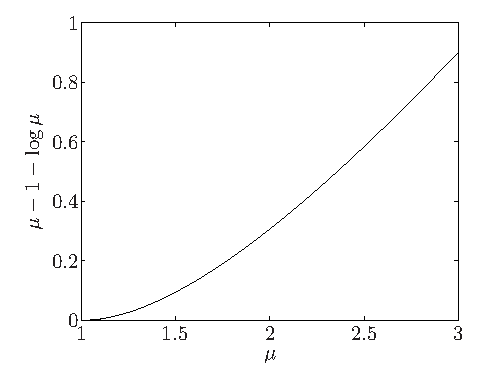
\includegraphics[width=.6\textwidth]{figures/ch11-13.pdf}
\caption*{图11.13 函数 $\mu-1-\log\mu$ 随 $\mu$ 的变化。障碍法一次外迭代所需牛顿步数的上界为 $(m/\gamma)(\mu-1-\log\mu)+c$。}
\end{figure}
结论是
\begin{equation}
\frac{m(\mu-1-\log\mu)}{\gamma}+c\tag{11.26}
\end{equation}
是 (11.25) 的上界，因此也是障碍法一次外迭代所需牛顿步数的上界。图11.13给出函数 $\mu-1-\log\mu$。$\mu$ 较小时，它近似二次增长；$\mu$ 很大时，它近似线性增长。这符合我们的直观：$\mu$ 接近 $1$ 时，中心化所需牛顿步数较少；$\mu$ 很大时，步数完全可能增加。

界 (11.26) 表明，每次中心化所需的牛顿步数，有一个主要取决于 $\mu$ 和 $m$ 的上界，其中 $\mu$ 是障碍法每次外迭代更新 $t$ 的倍数，$m$ 是问题的不等式约束数。它还弱依赖内迭代线搜索的参数 $\alpha$ 和 $\beta$，并以很弱的方式依赖内迭代的终止容差。有意思的是，这个界不依赖变量维数 $n$、等式约束数 $p$，也不依赖问题数据，即目标函数和约束函数的具体取值，前提是第11.5.1节的自协调性假设成立。最后，它不依赖 $t$；特别地，当 $t\to\infty$ 时，每次外迭代的牛顿步数仍有一致上界。

% Source PDF page 604 (printed p. 590)
\subsection{总牛顿迭代次数}
现在可以给出障碍法总牛顿步数的上界，不计初始中心化，后者将在第一阶段分析中讨论。将每次外迭代的牛顿步数上界 (11.26) 与外迭代次数 (11.13) 相乘，得到所需总牛顿步数的上界
\begin{equation}
N=\left\lceil\frac{\log(m/(t^{(0)}\epsilon))}{\log\mu}\right\rceil
\left(\frac{m(\mu-1-\log\mu)}{\gamma}+c\right).\tag{11.27}
\end{equation}
这一公式表明，自协调性假设成立时，对任意 $\mu>1$，都能界定障碍法所需的牛顿步数。

固定 $\mu$ 和 $m$ 时，上界 $N$ 与 $\log(m/(t^{(0)}\epsilon))$ 成正比。后者是初始对偶间隙 $m/t^{(0)}$ 与最终对偶间隙 $\epsilon$ 的比值的对数，即要求的对偶间隙缩减倍数的对数。因此可以说障碍法至少线性收敛，因为达到给定精度所需的步数，随精度倒数按对数增长。

固定 $\mu$ 与要求的对偶间隙缩减倍数时，上界 $N$ 随不等式数 $m$ 线性增长。它不依赖其他维数 $n,p$ 以及具体的问题数据或函数。下面将看到，按依赖 $m$ 的特定方式选择 $\mu$，可以使牛顿步数的上界仅按 $\sqrt m$，而不是按 $m$ 增长。

最后，考察上界 $N$ 随算法参数 $\mu$ 的变化。当 $\mu$ 趋近 $1$ 时，$N$ 中的第一项变大，因此 $N$ 变大。这与直观和观察相符：$\mu$ 接近 $1$ 时，外迭代次数很大。$\mu$ 很大时，上界 $N$ 近似按 $\mu/\log\mu$ 增长，这次是因为每次外迭代所需牛顿步数的上界增大。这同样与观察一致。因此，$N$ 作为 $\mu$ 的函数有最小值。

图11.14展示了上界随参数 $\mu$ 的变化，绘出了以下数值下 (11.27) 与 $\mu$ 的关系：
\[
c=6,\qquad\gamma=1/375,\qquad m/(t^{(0)}\epsilon)=10^5,\qquad m=100.
\]
该界在定性上符合直观和观察：$\mu$ 趋近 $1$ 时很大，$\mu$ 很大时则较慢地增大。$N$ 在 $\mu\approx1.02$ 处取最小值，此时总牛顿迭代次数的上界约为 $8000$。牛顿法的复杂度分析保守，但图中反映了选择 $\mu$ 的基本权衡。（实际中，大得多的 $\mu$，例如约 $2$ 至 $100$，都效果很好，总牛顿迭代次数只是几十次。）

\subsubsection*{将 $\mu$ 选为 $m$ 的函数}
固定 $\mu$ 及要求的对偶间隙缩减倍数时，界 (11.27) 随不等式数 $m$ 线性增长。将 $\mu$ 选为 $m$ 的函数，可以改善 $m$ 的幂指数。取
% Source PDF page 605 (printed p. 591)
\begin{equation}
\mu=1+1/\sqrt m.\tag{11.28}
\end{equation}
\begin{figure}[htbp]\centering
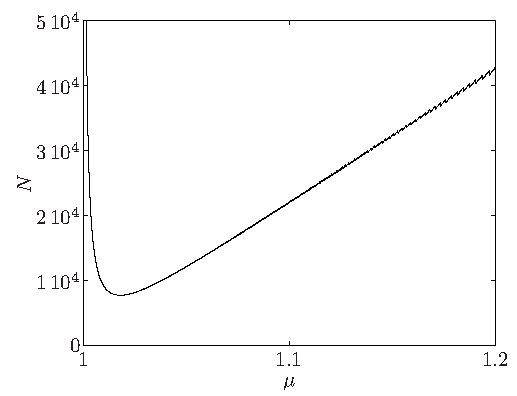
\includegraphics[width=.64\textwidth]{figures/ch11-14.pdf}
\caption*{图11.14 式 (11.27) 给出的总牛顿迭代次数上界 $N$ 与障碍算法参数 $\mu$ 的关系，其中 $c=6$、$\gamma=1/375$、$m=100$，对偶间隙缩减倍数 $m/(t^{(0)}\epsilon)=10^5$。}
\end{figure}
则 (11.27) 中的第二项满足
\begin{align*}
\mu-1-\log\mu&=1/\sqrt m-\log(1+1/\sqrt m)\\
&\le1/\sqrt m-1/\sqrt m+1/(2m)\\
&=1/(2m),
\end{align*}
这里使用 $a\ge0$ 时 $-\log(1+a)\le-a+a^2/2$。由对数的凹性，还有
\[
\log\mu=\log(1+1/\sqrt m)\ge(\log2)/\sqrt m.
\]
利用这些不等式，总牛顿步数的界为
\begin{equation}\begin{aligned}
N&\le\left\lceil\frac{\log(m/(t^{(0)}\epsilon))}{\log\mu}\right\rceil
\left(\frac{m(\mu-1-\log\mu)}\gamma+c\right)\\
&\le\left\lceil\frac{\sqrt m\log(m/(t^{(0)}\epsilon))}{\log2}\right\rceil
\left(\frac1{2\gamma}+c\right)\\
&=\left\lceil\sqrt m\log_2(m/(t^{(0)}\epsilon))\right\rceil
\left(\frac1{2\gamma}+c\right)\\
&\le c_1+c_2\sqrt m,
\end{aligned}\tag{11.29}\end{equation}
其中
\[
c_1=\frac1{2\gamma}+c,\qquad
c_2=\log_2(m/(t^{(0)}\epsilon))\left(\frac1{2\gamma}+c\right).
\]
% Source PDF page 606 (printed p. 592)
这里 $c_1$ 只弱依赖中心化牛顿步骤的算法参数，$c_2$ 还依赖要求的对偶间隙缩减倍数。注意，$\log_2(m/(t^{(0)}\epsilon))$ 正好是要求缩减对偶间隙的比特数。

固定对偶间隙缩减倍数时，界 (11.29) 按 $\sqrt m$ 增长，而若固定参数 $\mu$，(11.27) 中的上界 $N$ 按 $m$ 增长。因此，参数取 (11.28) 的障碍法称为 $\sqrt m$ 阶方法。

实际中不会采用 $\mu=1+1/\sqrt m$，因为这个值太小，甚至不会将 $\mu$ 选为随 $m$ 减小的函数。我们之所以关注这个 $\mu$，只是因为它近似最小化了那个非常保守的牛顿步数上界，并给出按 $\sqrt m$ 而非 $m$ 增长的总估计。

\subsection{可行性问题}
本节分析第11.4.1节基本第一阶段方法的一个小变体的复杂度，用它求解凸不等式组
\begin{equation}
f_1(x)\le0,\quad\ldots,\quad f_m(x)\le0,\tag{11.30}
\end{equation}
其中 $f_1,\ldots,f_m$ 为凸函数，具有连续的二阶导数。（等式约束留到后面考虑。）假设第一阶段问题
\begin{equation}\begin{aligned}
\text{最小化}\quad&s\\\text{约束为}\quad&f_i(x)\le s,\quad i=1,\ldots,m
\end{aligned}\tag{11.31}\end{equation}
满足第11.5.1节的条件。特别地，假设不等式组 (11.30) 的可行集（它当然可以为空）包含在半径为 $R$ 的欧氏球内：
\[
\{x\mid f_i(x)\le0,\ i=1,\ldots,m\}\subseteq\{x\mid\norm{x}_2\le R\}.
\]
可将 $R$ 解释为不等式组中任一可行点范数的先验界。这一假设意味着第一阶段问题的下水平集有界。不失一般性，以 $x=0$ 作为第一阶段方法的起点。定义 $F=\max_i f_i(0)$ 为最大约束违反程度，假设它为正，否则 $x=0$ 已满足 (11.30)。

用 $\bar p^\star$ 表示第一阶段优化问题 (11.31) 的最优值。$\bar p^\star$ 的符号决定不等式组 (11.30) 是否可行，其大小也有意义。如果 $\bar p^\star$ 为正且很大，例如接近它可能达到的最大值 $F$，则不等式组相当不可行：对每个 $x$，至少有一个不等式被明显违反，违反程度至少为 $\bar p^\star$。另一方面，若 $\bar p^\star$ 为负且绝对值很大，则不等式组相当可行：不仅存在 $x$ 使所有 $f_i(x)$ 非正，而且存在 $x$ 使所有 $f_i(x)$ 都是相当大的负数，不超过 $\bar p^\star$。因此，$|\bar p^\star|$ 衡量不等式组的可行性或不可行性有多明确，进而与
% Source PDF page 607 (printed p. 593)
判定 (11.30) 可行性的难度有关。特别地，若 $|\bar p^\star|$ 很小，意味着问题接近可行与不可行的分界。

为判定不等式组的可行性，采用基本第一阶段问题 (11.31) 的一个变体，增加冗余线性不等式 $a^\T x\le1$，得到
\begin{equation}\begin{aligned}
\text{最小化}\quad&s\\\text{约束为}\quad&f_i(x)\le s,\quad i=1,\ldots,m,\\&a^\T x\le1.
\end{aligned}\tag{11.32}\end{equation}
稍后给出 $a$。所选的 $a$ 将满足 $\norm{a}_2\le1/R$，于是 $\norm{x}_2\le R$ 蕴含 $a^\T x\le1$，即附加约束冗余。

选择 $a$ 和 $s_0$，使 $x=0$、$s=s_0$ 位于问题 (11.32) 的中心路径上，对应参数值 $t^{(0)}$，即它们最小化
\[
t^{(0)}s-\sum_{i=1}^m\log(s-f_i(x))-\log(1-a^\T x).
\]
令关于 $s$ 的导数为零，得到
\begin{equation}
t^{(0)}=\sum_{i=1}^m\frac1{s_0-f_i(0)}.\tag{11.33}
\end{equation}
令关于 $x$ 的梯度为零，得到
\begin{equation}
a=-\sum_{i=1}^m\frac1{s_0-f_i(0)}\nabla f_i(0).\tag{11.34}
\end{equation}
因此只剩参数 $s_0$ 尚需选择。选定后，向量 $a$ 由 (11.34) 给出，参数 $t^{(0)}$ 由 (11.33) 给出。由于 $x=0$、$s=s_0$ 必须对第一阶段问题 (11.32) 严格可行，必须取 $s_0>F$。

还必须选择 $s_0$，保证 $\norm{a}_2\le1/R$。由 (11.34)，
\[
\norm{a}_2\le\sum_{i=1}^m\frac1{s_0-f_i(0)}\norm{\nabla f_i(0)}_2\le\frac{mG}{s_0-F},
\]
其中 $G=\max_i\norm{\nabla f_i(0)}_2$。因此可取 $s_0=mGR+F$，使 $\norm{a}_2\le1/R$，从而附加线性不等式冗余。

利用 (11.33)，有
\[
t^{(0)}=\sum_{i=1}^m\frac1{mGR+F-f_i(0)}\ge\frac1{mGR},
\]
因为 $F=\max_i f_i(0)$。于是 $x=0$、$s=s_0$ 位于第一阶段问题 (11.32) 的中心路径上，其初始对偶间隙满足
\[
\frac{m+1}{t^{(0)}}\le(m+1)mGR.
\]

% Source PDF page 608 (printed p. 594)
为求解原不等式组 (11.30)，需要判定 $\bar p^\star$ 的符号。当 (11.32) 的原始目标值为负，或对偶目标值为正时即可停止。当 (11.32) 的对偶间隙小于 $|\bar p^\star|$ 时，必然出现这两种情况之一。

用障碍法求解 (11.32)，从对偶间隙不超过 $(m+1)mGR$ 的中心点出发，在对偶间隙小于 $|\bar p^\star|$ 时或之前终止。利用前一节的结果，所需牛顿步数不超过
\begin{equation}
\left\lceil\sqrt{m+1}\log_2\frac{m(m+1)GR}{|\bar p^\star|}\right\rceil
\left(\frac1{2\gamma}+c\right).\tag{11.35}
\end{equation}
这里取 $\mu=1+1/\sqrt{m+1}$，它比固定 $\mu$ 能给出更好的 $m$ 的复杂度指数。

界 (11.35) 的增长只略快于 $\sqrt m$，并且弱依赖中心化步骤的算法参数。它近似与 $\log_2((GR)/|\bar p^\star|)$ 成正比，可将后者解释为具体可行性问题的难度，或它距可行与不可行分界的接近程度。

\subsubsection*{含等式约束的可行性问题}
通过消去等式约束，同样的分析可用于含等式约束的可行性问题。消元不影响自协调性，但此时 $G$ 与 $R$ 指的是约化后，即消元后的问题。

\subsection{第一阶段与第二阶段的合并复杂度}
本节对使用障碍法的一个变体求解问题
\[
\begin{aligned}\text{最小化}\quad&f_0(x)\\\text{约束为}\quad&f_i(x)\le0,\quad i=1,\ldots,m,\\&Ax=b\end{aligned}
\]
给出从头到尾的复杂度分析。首先求解第一阶段问题
\[
\begin{aligned}
\text{最小化}\quad&s\\
\text{约束为}\quad&f_i(x)\le s,\quad i=1,\ldots,m,\\
&f_0(x)\le M,\\&Ax=b,\\&a^\T x\le1,
\end{aligned}
\]
假设它满足第11.5.1节的自协调性与下水平集有界假设。这里在基本第一阶段问题中加了两个冗余不等式。加入约束 $f_0(x)\le M$，是为了保证第一阶段的中心路径与第二阶段中心路径相交，正如第11.4.1节描述的那样，见 (11.21)。$M$ 是问题最优值的先验界。第二个新增约束为线性不等式 $a^\T x\le1$，其中 $a$ 按
% Source PDF page 609 (printed p. 595)
第11.5.4节选取。用障碍法求解这一问题，取 $\mu=1+1/\sqrt{m+2}$，初始点 $x=0$、$s=s_0$ 按第11.5.4节给出。

找到严格可行点或确定问题不可行，所需牛顿步数不超过
\begin{equation}
N_{\mathrm I}=\left\lceil\sqrt{m+2}\log_2\frac{(m+1)(m+2)GR}{|\bar p^\star|}\right\rceil
\left(\frac1{2\gamma}+c\right),\tag{11.36}
\end{equation}
其中 $G$ 与 $R$ 见第11.5.4节。如果问题不可行，算法结束；如果问题可行，则在第一阶段找到与 $s=0$ 对应的点，它位于第二阶段问题
\[
\begin{aligned}
\text{最小化}\quad&f_0(x)\\
\text{约束为}\quad&f_i(x)\le0,\quad i=1,\ldots,m,\\
&Ax=b,\\&a^\T x\le1
\end{aligned}
\]
的中心路径上。该初始点对应的初始对偶间隙不超过 $(m+1)(M-p^\star)$，见 (11.22)。假设第二阶段问题也满足第11.5.1节的自协调性与下水平集有界假设。

现在进入第二阶段，仍使用障碍法。必须将对偶间隙从不超过 $(m+1)(M-p^\star)$ 的初值降低到某个容差 $\epsilon>0$，至多需要
\begin{equation}
N_{\mathrm{II}}=\left\lceil\sqrt{m+1}\log_2\frac{(m+1)(M-p^\star)}{\epsilon}\right\rceil
\left(\frac1{2\gamma}+c\right)\tag{11.37}
\end{equation}
个牛顿步。

因此总牛顿步数不超过 $N_{\mathrm I}+N_{\mathrm{II}}$。该界随不等式数 $m$ 近似按 $\sqrt m$ 增长，并包含依赖具体问题实例的两项
\[
\log_2\frac{GR}{|\bar p^\star|},\qquad\log_2\frac{M-p^\star}{\epsilon}.
\]

\subsection{小结}
本节的复杂度分析主要有理论意义。特别提醒读者，本节讨论的 $\mu=1+1/\sqrt m$ 在实际中是很差的选择；它唯一的优点，是得到按 $\sqrt m$ 而非 $m$ 增长的界。同样，实际中也不推荐增加冗余不等式 $a^\T x\le1$。

由上述分析得到的实际数值界远高于观察到的迭代次数。甚至界的阶数似乎也保守。最好的牛顿步数界按 $\sqrt m$ 增长，而实际经验表明，牛顿步数几乎不随 $m$，实际上也几乎不随任何其他参数增长。

不过，知道自协调性条件成立时，可以为障碍法每次中心化
% Source PDF page 610 (printed p. 596)
所需的牛顿步数给出一致上界，仍然让人放心。障碍法一个明显的潜在问题是：随着 $t$ 增大，对应的中心化问题可能越来越难，需要更多牛顿步。虽然实际经验表明并非如此，一致上界进一步增强了我们对其不会发生的信心。

最后指出，重新表述问题使其满足自协调性条件，是否能带来实际优势，目前尚不清楚。只能说，自协调性条件成立时，障碍法在实践中会很好地工作，而且可以给出最坏情况复杂度界。
